
\chapter{PID Control in Simulation Environment}

The primary goal of this thesis project is to create a vehicle that satisfies the needs of the GDCS coral monitoring projects. Specifically, the uDrone needs to be able to follow the contour of the reef at a set distance. In order to show that this is possible, a simulation environment was developed that shows this capability. The details of how this simulation environment was created and the results are detailed in this section.\footnote{The software for this application was written jointly by the author and A.L.G. Prasad, another member of the DREAMS Lab who is working on uDrone autonomy. Help and code snippets were also provided by Harish Anand, another DREAMS Lab member.} 

\section{Methods}

This trial features a simulated uDrone following the terrain contours of a known reef profile. In order to do this, a simulation environment was built, a controller was developed and a contour profile was measured.  

\subsection{Simulation Environment Setup}

A world was created in Gazebo that contained a reef model. In this case, the reef model obtained by me using 3D motion capture while scuba diving was used. The model was scaled to a near realistic size. The world not only has the reef topography but also as a photographic overlay of the reef. UUV sim was also used in the simulated world. This allowed for mimicking some of the characteristics of water, such as buoyant forces and hydrodynamic damping. 

The uDrone model was added to the word file. This particular uDrone model was outfit with a downward-facing, broad-beam, sonar. The particular sonar used was the hector gazebo sonar plugin \parencite{sonar}. The specifications of the simulated sonar are set up to match the Blue Robotics Ping Echosounder used in the actual uDrone. This meant a beam-width of 30 degrees was used.

An emulated instance of the PX4 flight stack was used for the direct motor control of the uDrone. This was done using the PX4 Software in the Loop (SITL) for simulation where the PX4 software is run on a software emulated flight controller. The air-frame configuration of the HippoCampus \textmu AUV was used as it very closely mimics the motor configuration of the uDrone. The MAVROS plugin for ROS was used to communicate with the PX4 flight stack over MAVLink. 

\subsection{ROS Setup}
\begin{figure}[h]
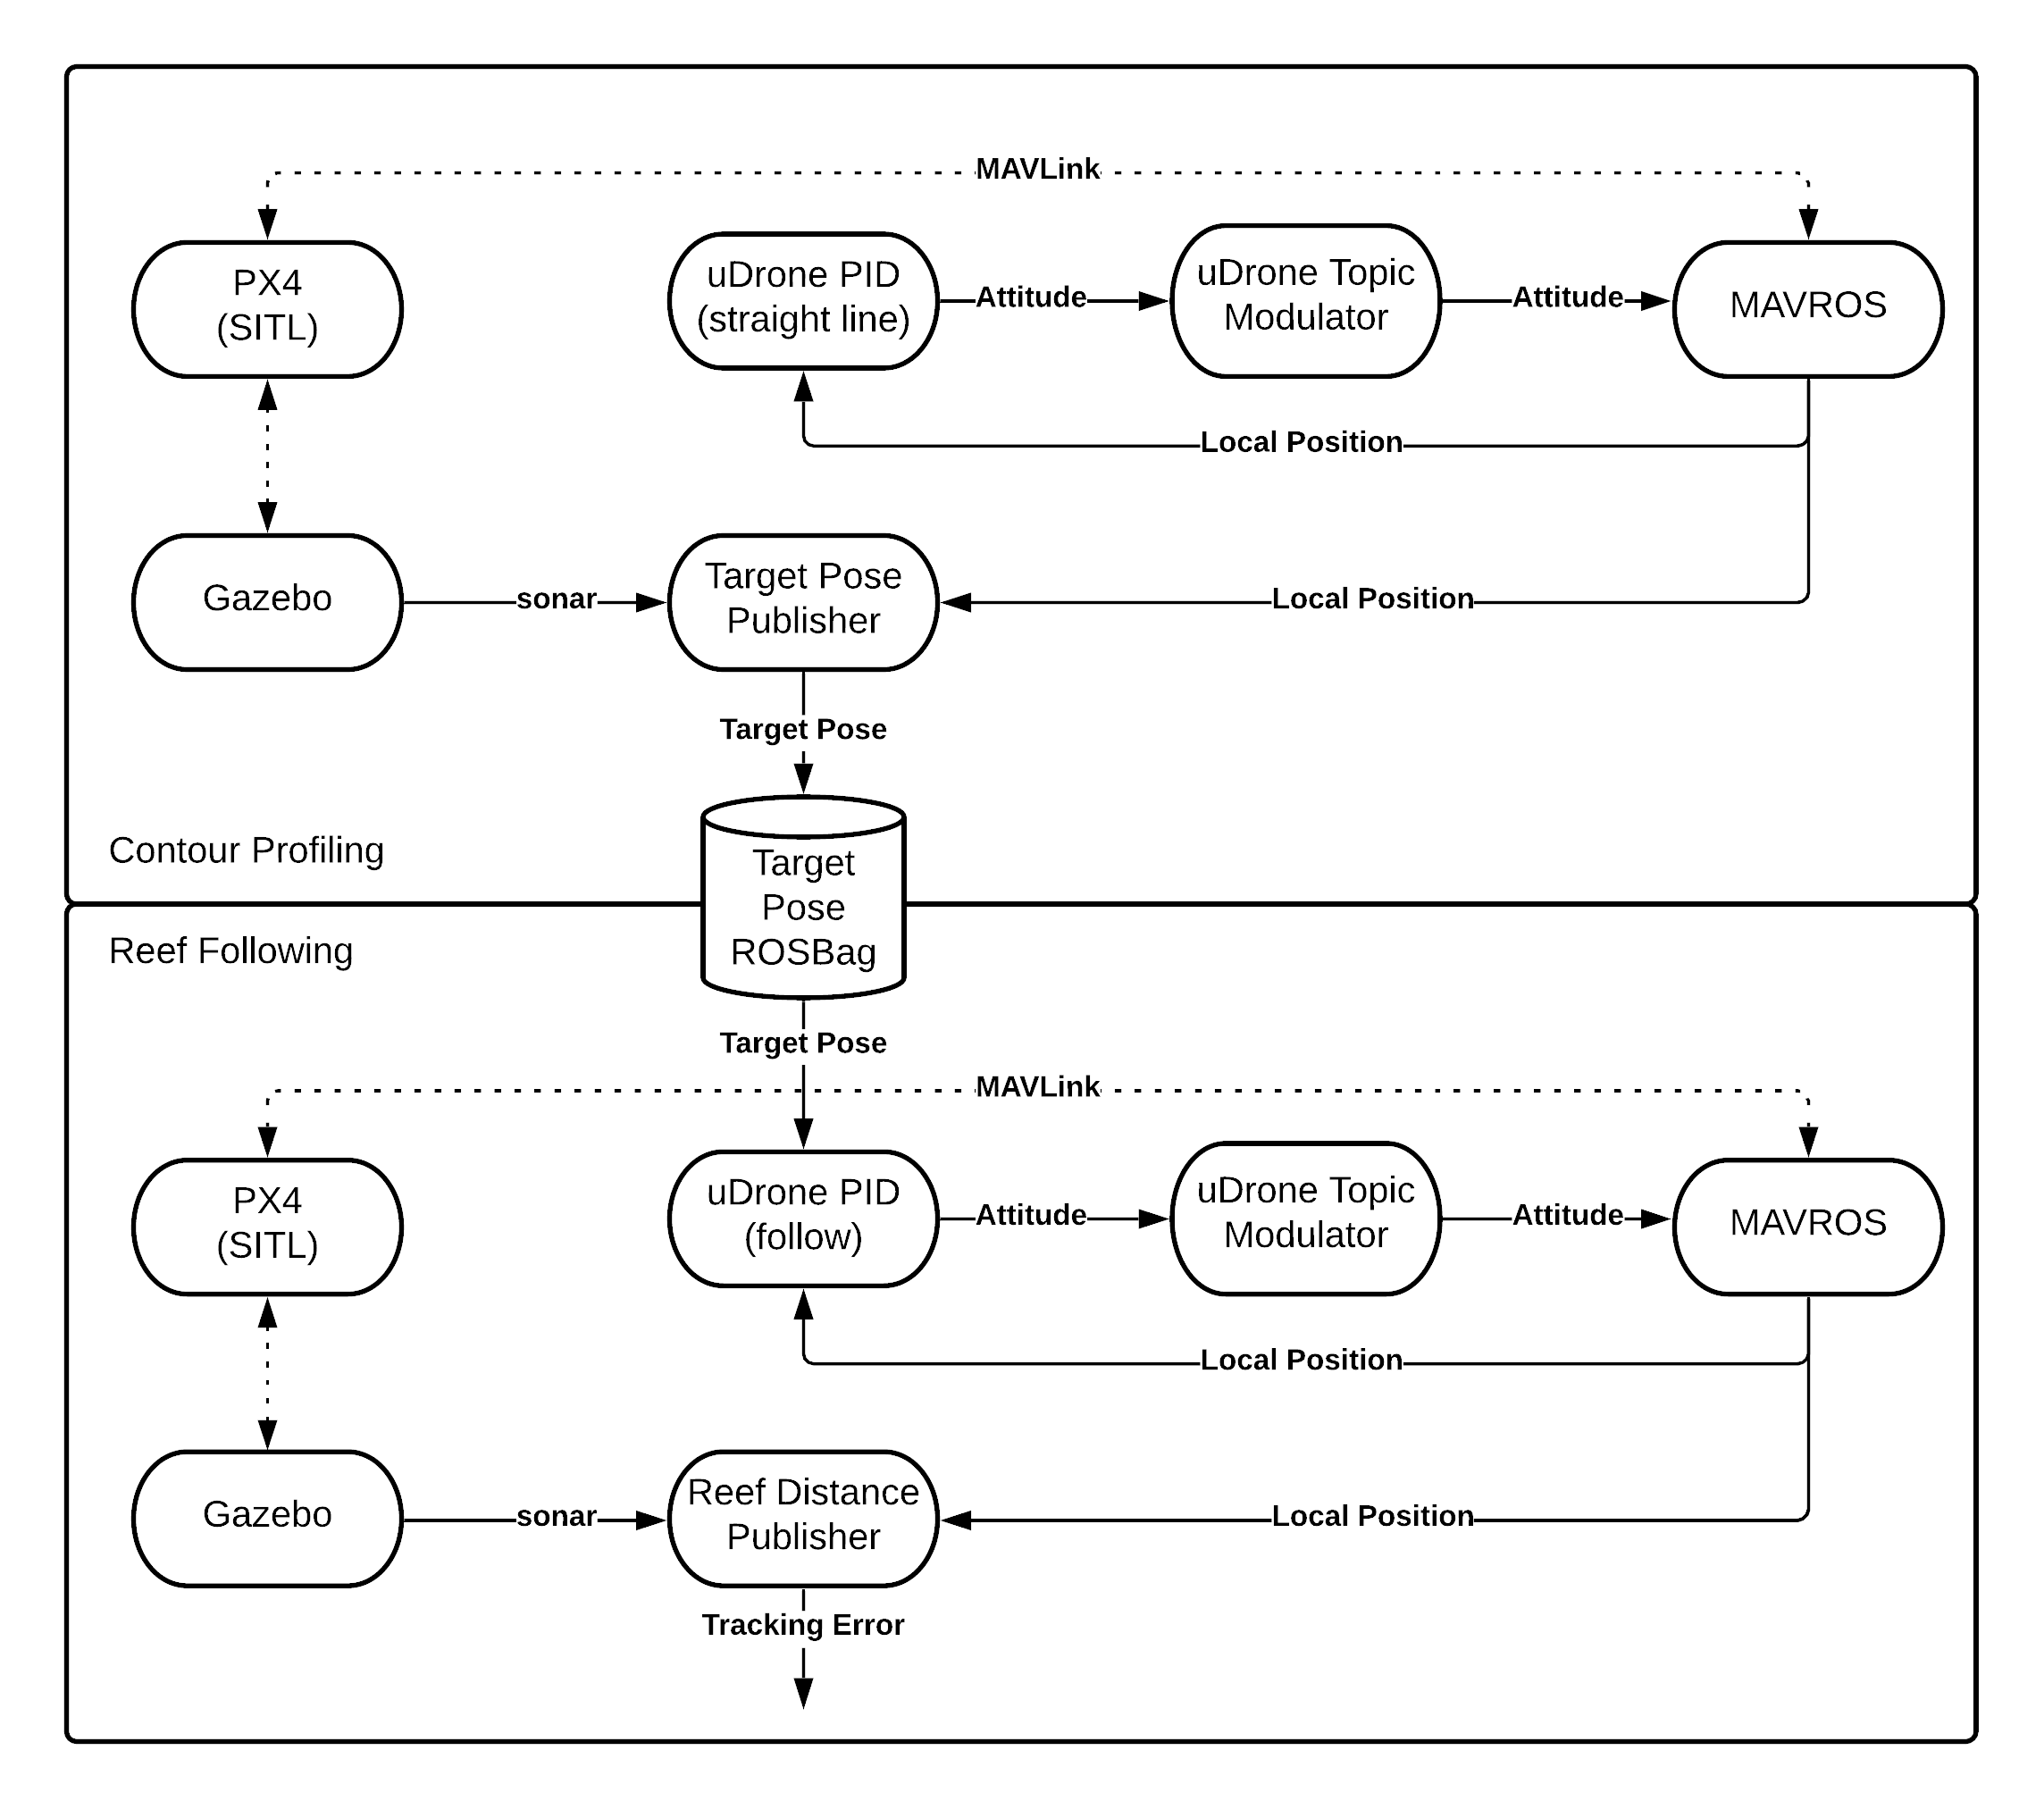
\includegraphics[width=\maxwidth{\textwidth}]{img/ros.png}
\caption{ROS Nodes for Contour Profiling and Reef Following in Simulation}
\label{ros}
\end{figure}

The program was broken into nodes following the ROS development model. The diagram of the node layout can be seen in figure \ref{ros}.

A special ROS node was created, called the uDrone Topic Modulator, in order to launch all of these components together and communication with the uDrone through MAVROS. This startup node’s launch file loaded the reef and uDrone into the Gazebo simulation and initiated PX4 SITL. A C++ program written as part of this node connected to the vehicle set the flight mode to “offboard,” and armed the vehicle. This process was necessary for the controller to begin sending messages over MAVLink to the uDrone for control. It also listened for commands from other nodes and sent them along to the uDrone via MAVROS. 

The PID controller was a separate node that took in the uDrone's local position via MAVROS along with a target position and pose. This node had two modes. In follow mode it listened for a target pose and then followed it. In contour profiling mode it followed a path set in the C++ code. The path used for this application was a straight line. The PID controller itself will be discussed in section \ref{controller}. 

A final node was developed that served two purposes, depending on the need. This is called the Target Pose Publisher or Reef Distance Publisher. This node took in the sonar data output from the simulated echosounder in Gazebo along with the local position from MAVROS. In the contour profiling cases it output the target pose, as described in section \ref{contour}.In the reef following case it output the tracking error, or distance to the reef, used to calculate the results in section \ref{pid-results}.

The element that connects the contour profiling with the reef following is a ROSBag. The ROSBag packages is a built in feature of ROS that allows for the recording of data while ROS is running. In this case it was used to record the target pose from the contour profiling run. Then it was played back during the reef following run in order to send the uDrone the desired pose and position. 

\subsection{Controller Development}\label{controller}

For this application, a proportional–integral–derivative (PID) controller was developed to control the movement of the uDrone. While the PID is developed as a single controller, it controls the position in all three directions independently. The proportional term was found by comparing the desired position to the local position, as reported by the internal position estimator in PX4. This local position is relative to the vehicles starting point and determined using an extended Kalman filter that fuses data from the PixHawks internal IMU, Gyroscope, and compass. The proportional gain is set to 0.5. The integral term is found by summing past proportional errors. In this case, only the past two errors are summed and the gain is set to 0.005. The derivative term is estimated by calculating the change in error from the last time-step to this time-step and dividing by the step size. The gain for the derivative term is 0.05. 

The PID controller outputs a vector with a direction and magnitude, essentially pointing towards where the vehicle should go and how fast it should go there. In order to convert this into a usable control the method from \cite{faf} is used.

\section{Contour profiling}\label{contour}

A trajectory for reef following needed to be developed in order to accomplish this task. To do this, the simulation environment was started in the same way as for the final trial. However, instead of following a reef relative path, the uDrone was given the desired path of a straight line across the reef. As the uDrone traversed the reef, it took samples of the distance to the reef using the sonar. The final reef following path would follow the same trajectory on the X-Y plane as this straight line uDrone run. At each of these X and Y points, a new depth (Z) was recorded for the desired location. This point was calculated by subtracting the sonar depth value from the local depth value and then adding one. In the end, a trajectory was calculated and recorded that followed the reef at a distance of one meter. 

\subsection{Reef Following}

Another instance of the simulation was initiated, with the uDrone starting in the same spot relative to the reef as in the previous, contour profiling, step. The PID controller node, in this case, listened for the trajectory on a ROS topic. As desired set-points were received the controller instructed the uDrone on how to move through MAVROS. Meanwhile, the sonar readings were recorded in order to analyze the reef following the performance. 

Figure \ref{follow_ss} shows the uDrone moving over the reef in simulation. The vehicle can be observed pitched up to follow the reef. The blue cone below it is a visual representation of the sonar sensor which outputs the distance to the reef. 

\begin{figure}[ht]
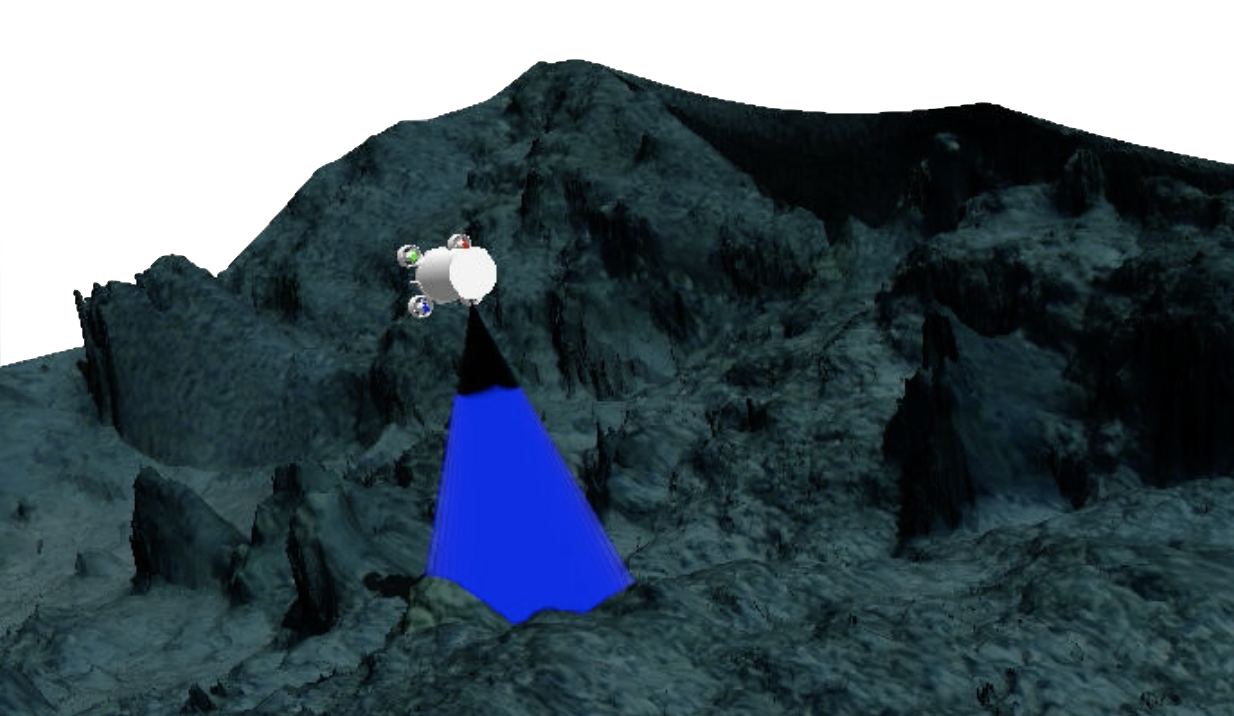
\includegraphics[width=\maxwidth{\textwidth}]{img/follow_ss.png}
\caption{uDrone During Reef Following in Simulation}
\label{follow_ss}
\end{figure}

\section{Results}\label{pid-results}

The uDrone was able to follow the profile of the reef as measured by the initial reef mapping. Figure \ref{follow} shows the results of this trial. The blue line is the path of the uDrone relative to it initial location. The gray line is the sonar reading which is the distance from the uDrone to the reef. Using these two together, the orange line is obtained, which is the position of the reef relative to the uDrone. The data starts at the 1m point, because it takes the uDrone some time and distance to reach a cruising altitude relative to the reef. 

\begin{figure}[h]
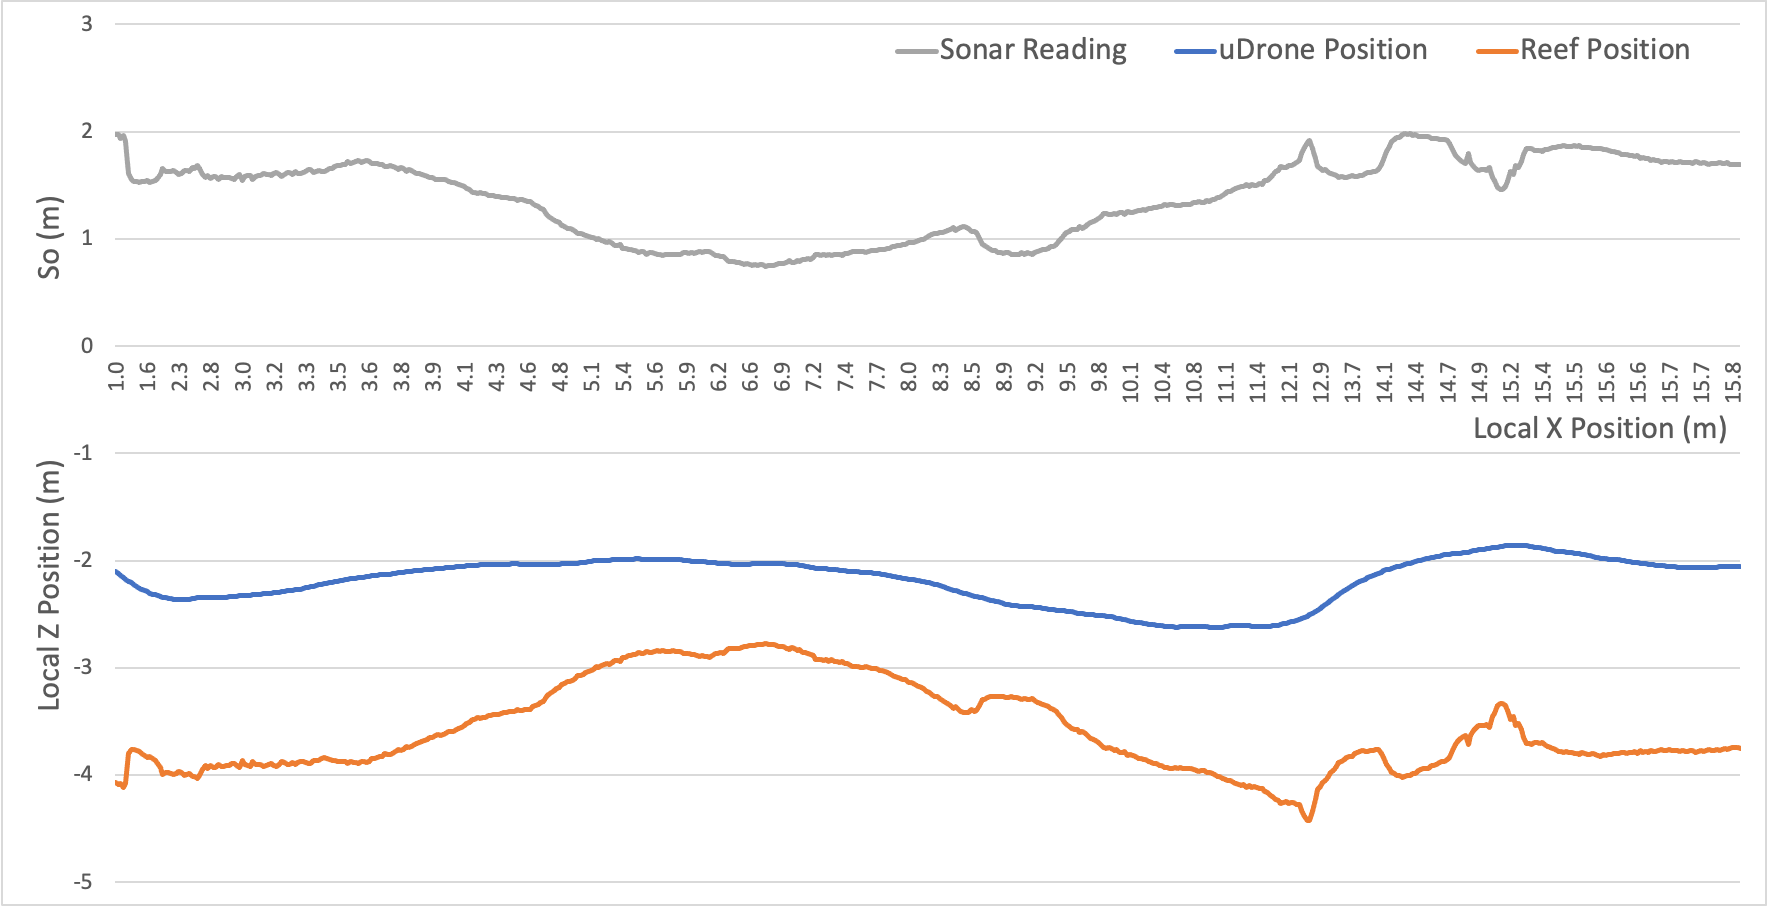
\includegraphics[width=\maxwidth{\textwidth}]{img/follow.png}
\caption{uDrone Reef Following Path and Sonar Reading}
\label{follow}
\end{figure}

As is shown in figure \ref{error}, the mean squared error is typically below 0.4. It gets as low as 0.15 as the vehicle spends more time at the desired height between the five and ten meter mark.  

\begin{figure}[h]
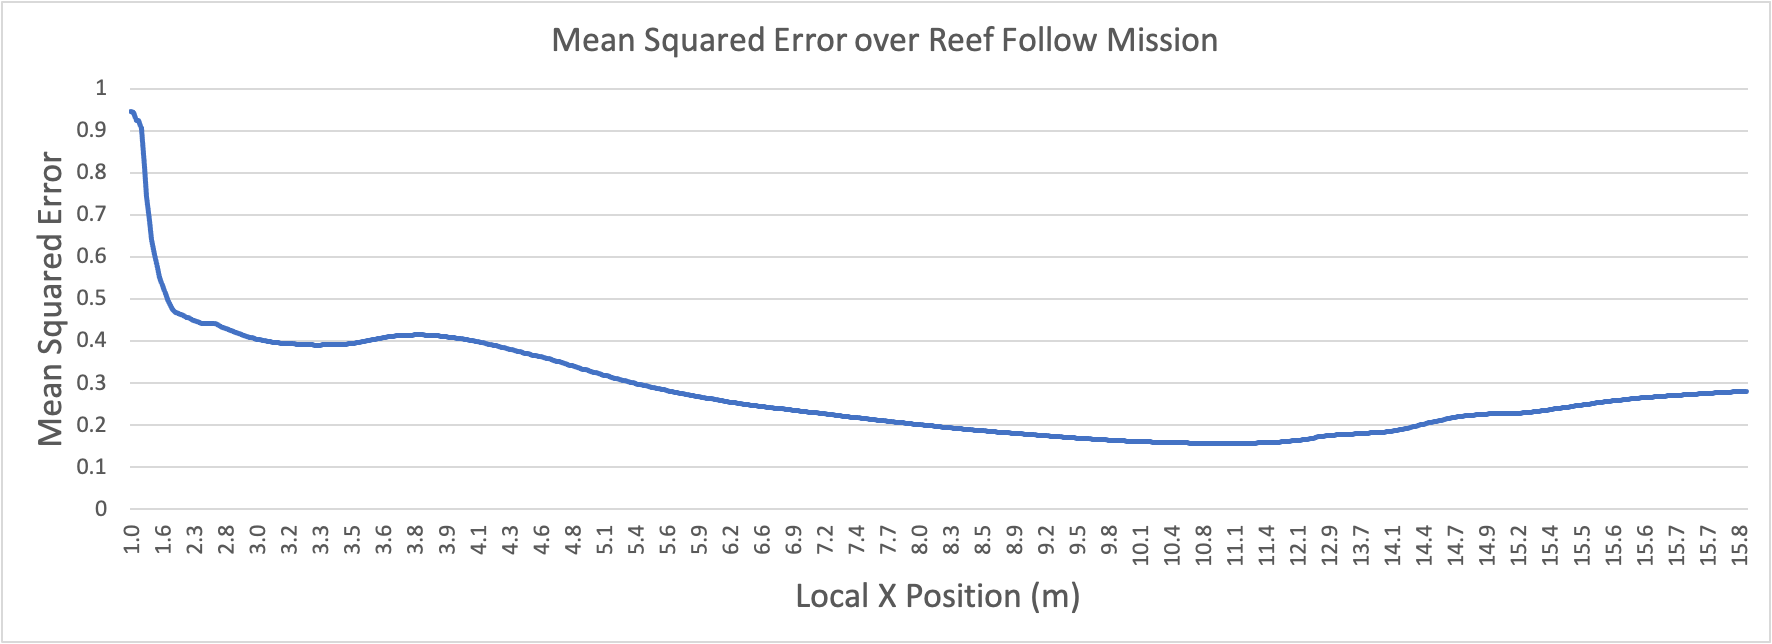
\includegraphics[width=\maxwidth{\textwidth}]{img/error.png}
\caption{Mean Squared Error over Reef Follow Mission}
\label{error}
\end{figure}
One major source of error in this method is the sonar. The sonar projects a cone and then averages the distance over that cone projection. This means the initial pass, which was roughly one meters above the reef, took a scan of a larger section of the reef than the follow pass. This means the desired location was based on the average distance to the reef of a bigger segment of the reef than that recorded when only one meter above the reef.

Another source of error is the PID controller itself. The tuning of this controller will effect how closely the vehicle stays to its desired path. While the uDrone PID was tuned so that it would generally work, it might not be the optimal tuning parameters.  

\section{Conclusion}

This experiment demonstrated that it is possible for the uDrone to practice reef following maneuvers with a PID controller and a known reef segment. As reef morphology data is collected for sections of reef, this method becomes more and more practical. Better resolution data for depth at various points will allow for even better results.

There are, however, drawbacks that would limit this approaches usefulness in a real world setting. First, localizing underwater is a difficult problem due to the lack of GPS. Therefore, it will be hard to start the uDrone from a known location relative to the reef from one trial to the next. This could be mitigated by using buoy to set start points, but that may requires adding man-made equipment to the reef. Second, this method relies on dead reckoning with the internal IMU to determine location. The error in the IMUs selected for the uDrone to not allow for dead reckoning over long distances, so some other method for localization must be used. And third, the reef is comprised of living organisms which may between trial times. The ideal situation is for the vehicle to use vision in real time to determine its path.